\documentclass[13pt]{article}
\usepackage[utf8]{inputenc}

\usepackage{polski}
\usepackage{pgfplots}
\usepackage{booktabs} 

\begin{document}
 
\begin{titlepage}
\begin{center}

\includegraphics[scale=1.0]{./Pwr_logo/logo_PWr_2.png}
\\
\vspace{1.5cm}
{\Huge Marcin Karasiewicz}
\\
\begin{Large}
\vspace{1.0cm}
Projektowanie algorytmów \\ i metody sztucznej inteligencji \\
\vspace{1.0cm}
Algorytmy sortowania
\end{Large}
\end{center}
\newpage
\tableofcontents 
\end{titlepage}
\newpage

\section{Algorytm Merge Sort }
\subsection{Opis}
Sortowanie przez scalanie jest przykładem algorytmu rekurencyjnego o złożoności $O(n\log{}n)$. Algorytm wykorzystuje metodę "dziel i zwyciężaj". Nasza nieposortowana tablica zostaje podzielona na dwie części. Rozkład tablic następuje rekurencyjnie aż tablice staną się jednoelementowe. Następnie tablice zostają złączone w szeregu posortowanym.
\subsection{Tabela pomiarów}

\begin{center}
\begin{tabular}{lcccc}  
\\
\toprule
Rozmiar[n] & \multicolumn{4}{c}{Czas[s]} \\
\cmidrule(r){2-5}
 & Losowe & Posortowane & O-Posortowane & Identyczne \\
\midrule
10       & 0.0000004616   & 0.0000006574 & 0.0000007159  & 0.0000006544 \\
100      & 0.0000040008   & 0.0000051883 & 0.0000064687  & 0.0000065753 \\
1000     & 0.0000609885   & 0.0000638151 & 0.0000839588  & 0.0001058314 \\
10000    & 0.0005665224   & 0.0005789379 & 0.0021117148  & 0.0008403904 \\
100000   & 0.0090663026   & 0.0062508104 & 0.0096813096  & 0.0060969113 \\
1000000  & 0.1338663745   & 0.0606525145 & 0.0814999795  & 0.0810095399 \\
10000000 & 0.8017014327   & 0.7031141995 & 0.7495614558  & 0.6749413904 \\
\bottomrule
\end{tabular}
\end{center}

\subsection{Wykres}

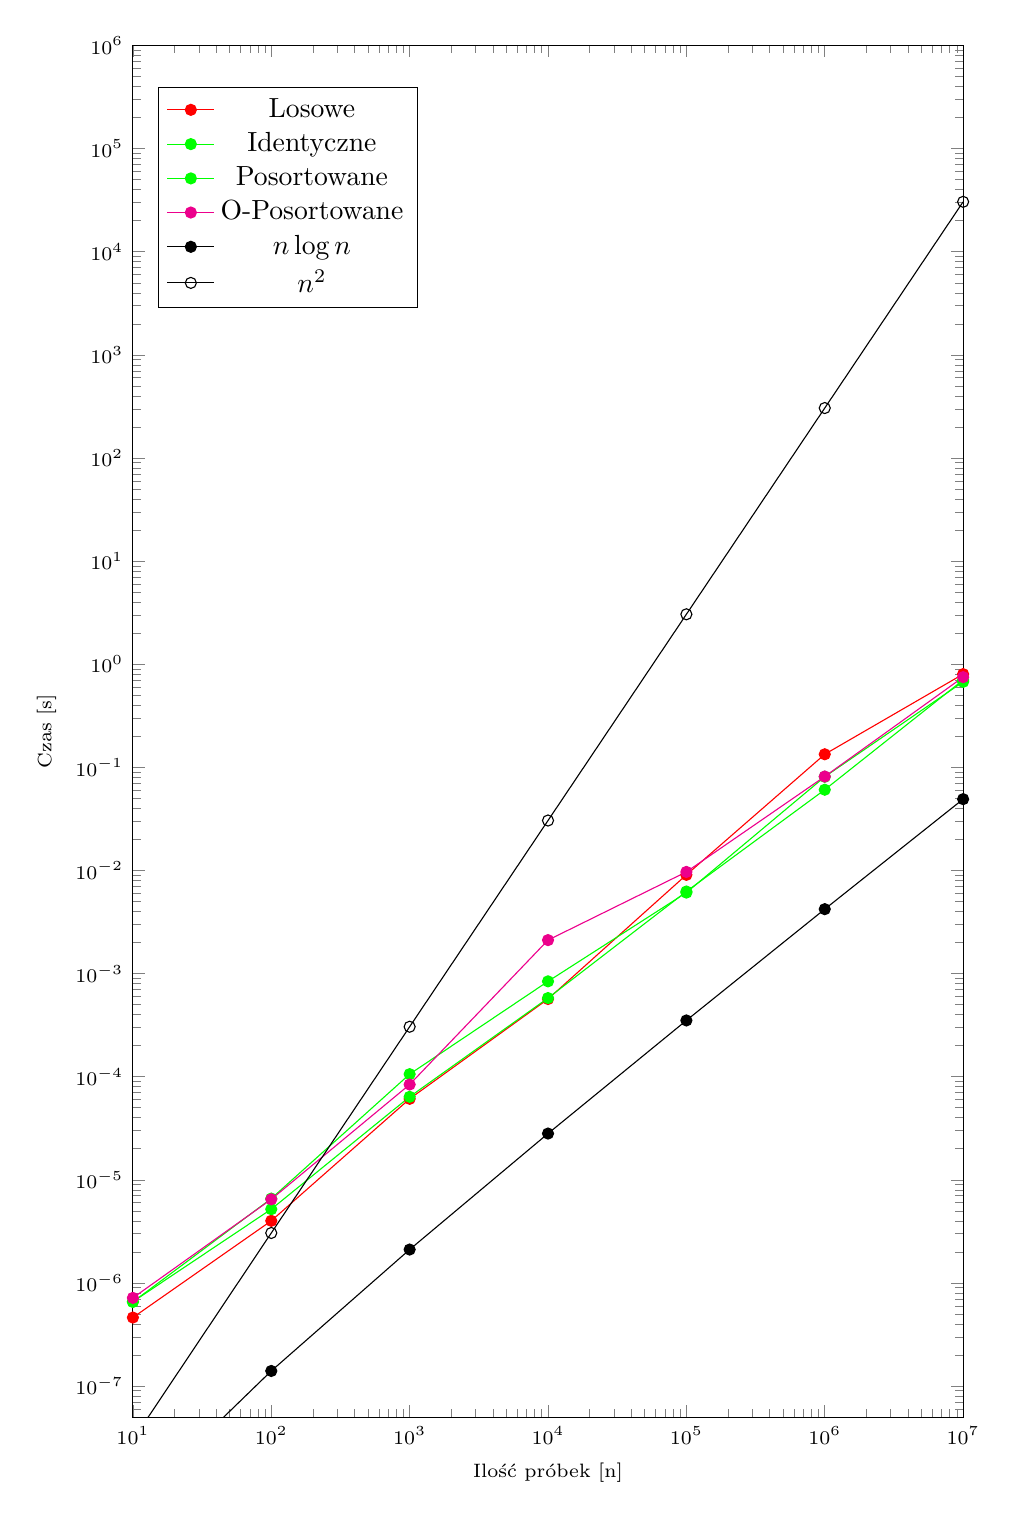
\begin{tikzpicture}
\\
\begin{axis}[
    width=\textwidth,
    height=19cm,
    legend pos=north west,
	xmode = log,
	ymode = log,
	xlabel={Ilość próbek [n]},
	ylabel={Czas [s]},
	xmin=10,xmax=10000000,
	ymin= 0.00000005, ymax=1000000,
	label style={font=\scriptsize},
	tick label style={font=\scriptsize},
	minor y tick num=1
]

\addplot[color=red,mark=*]
coordinates {
(10,0.0000004616 )
(100,0.0000040008)
(1000,0.0000609885)
(10000,0.0005665224)
(100000,0.0090663026)
(1000000,0.1338663745)
(10000000,0.8017014327)
};

\addplot[color=green,mark=*]
coordinates {
(10,0.0000006544 )
(100,0.0000065753)
(1000,0.0001058314)
(10000,0.0008403904)
(100000,0.0060969113)
(1000000,0.0810095399)
(10000000,0.6749413904)
};

\addplot[color=green,mark=*]
coordinates {
(10,0.0000006574 )
(100,0.0000051883)
(1000,0.0000638151)
(10000,0.0005789379)
(100000,0.0062508104)
(1000000,0.0606525145)
(10000000,0.7031141995)
};

\addplot[color=magenta,mark=*]
coordinates {
(10,0.0000007159 )
(100,0.0000064687)
(1000,0.0000839588)
(10000,0.0021117148)
(100000,0.0096813096)
(1000000,0.0814999795)
(10000000,0.7495614558)
};

\addplot[color=black,mark=*]
coordinates {
(10,0.000000007 )
(100,0.000000140)
(1000,0.000002107)
(10000,0.000028091)
(100000,0.000351138)
(1000000,0.004213657)
(10000000,0.049159335)
};

\addplot[color=black,mark=o]
coordinates {
(10,0.000000030 )
(100,0.000003050)
(1000,0.000304995)
(10000,0.030499469)
(100000,3.049946857)
(1000000,304.994685714)
(10000000,30499.468571429)
};

\legend{Losowe, Identyczne,Posortowane, O-Posortowane, $n\log{}n$,$n^2$}
\end{axis}
\end{tikzpicture}

\section{Algorytm Quick Sort }
Algorytm wykorzystuje technikę "dziel i zwyciężaj". Według ustalonego schematu wybierany jest jeden element w sortowanej tablicy nazywany Pivotem. W algorytmie zaimplementowanym na potrzeby kursu użyto techniki "median of three". Następnie ustawiamy elementy nie większe na lewo tej wartości, natomiast nie mniejsze na prawo. W ten sposób powstaną nam dwie części tablicy, gdzie w pierwszej części znajdują się elementy nie większe od drugiej. Następnie każdą z tych podtablic sortujemy osobno według tego samego schematu. Przypadek optymistyczny ma złożoność $O(n\log{}n)$, natomisat pesymistyczny który dało się wyeliminować po przez technikę "median od three" ma złożoność $O(n^2)$
\subsection{Opis}
\subsection{Tabela pomiarów}

\begin{center}
\begin{tabular}{lcccc} 
\\ 
\toprule
Rozmiar[n] & \multicolumn{4}{c}{Czas[s]} \\
\cmidrule(r){2-5}
 & Losowe & Posortowane & O-Posortowane & Identyczne \\
\midrule
10       & 0.0000002496  & 0.0000002133  & 0.0000002772  & 0.0000002119 \\
100      & 0.0000023181  & 0.0000011925  & 0.0000019025  & 0.0000016491 \\
1000     & 0.0000357067  & 0.0000123955  & 0.0000195050  & 0.0000313642 \\
10000    & 0.0003523159  & 0.0002506793  & 0.0002486864  & 0.0001850952 \\
100000   & 0.0048754355  & 0.0024690919  & 0.0031532092  & 0.0023649113 \\
1000000  & 0.0530444570  & 0.0226112096  & 0.0342633065  & 0.0343200958 \\
10000000 & 0.4847639445  & 0.2607655615  & 0.2432170252  & 0.2907808971 \\
\bottomrule
\end{tabular}
\end{center}

\subsection{Wykres}

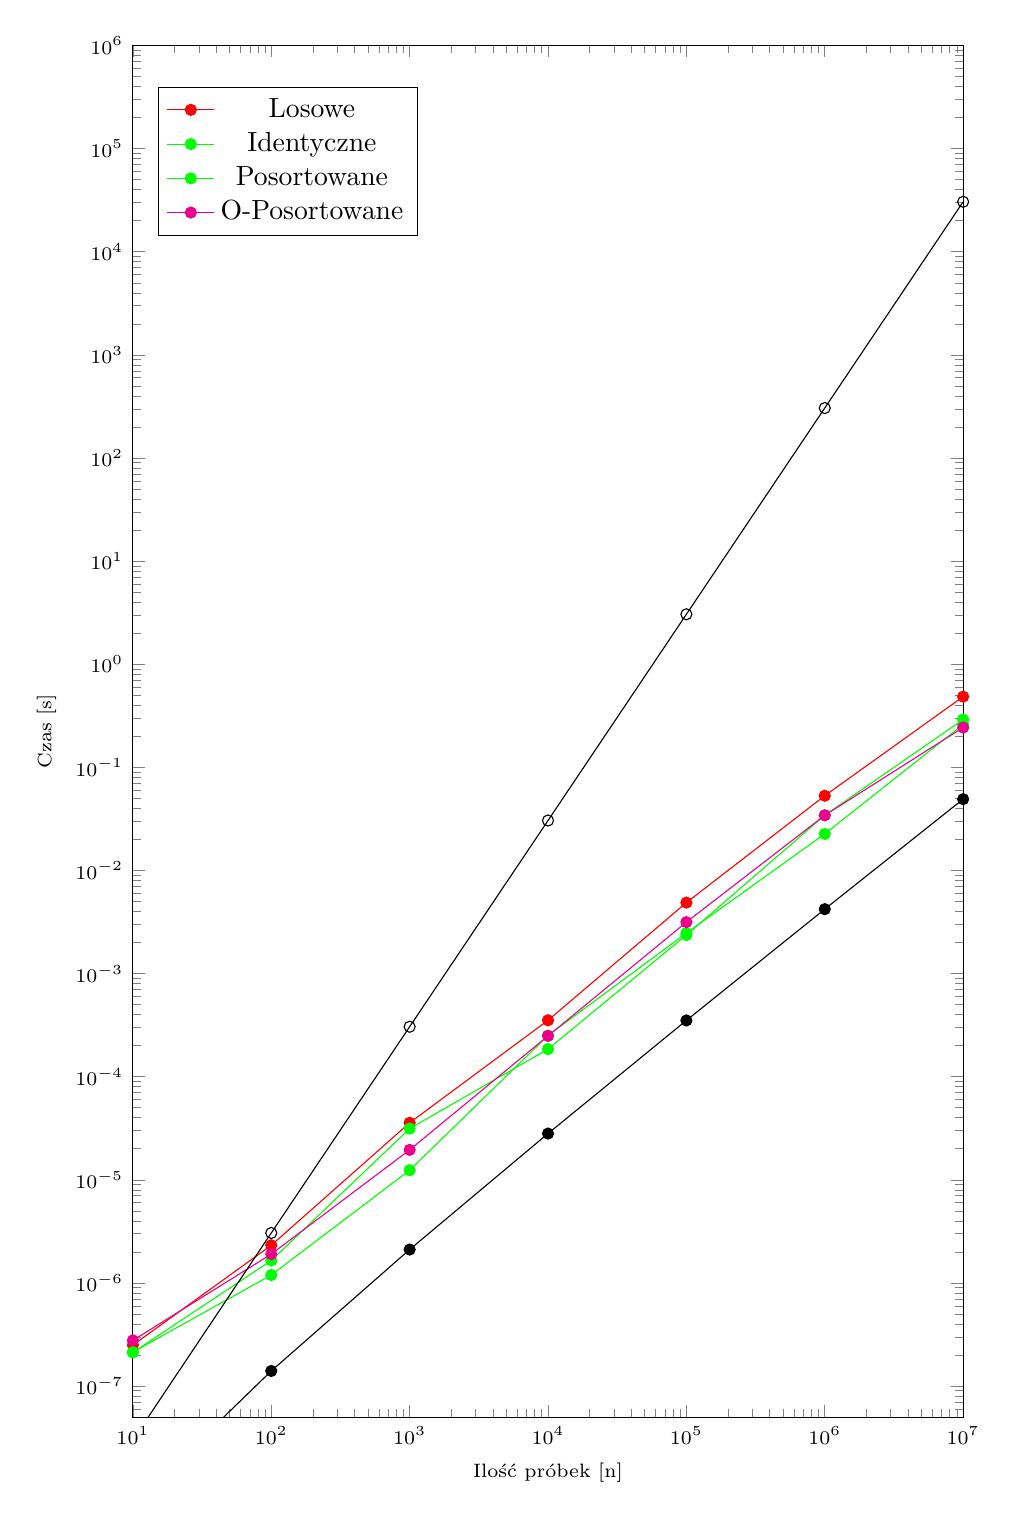
\begin{tikzpicture}
\\
\begin{axis}[
    width=\textwidth,
    height=19cm,
    legend pos=north west,
	xmode = log,
	ymode = log,
	xlabel={Ilość próbek [n]},
	ylabel={Czas [s]},
	xmin=10,xmax=10000000,
	ymin= 0.00000005, ymax=1000000,
	label style={font=\scriptsize},
	tick label style={font=\scriptsize},
	minor y tick num=1
]

\addplot[color=red,mark=*]
coordinates {
(10,0.0000002496 )
(100,0.0000023181)
(1000,0.0000357067)
(10000,0.0003523159)
(100000,0.0048754355)
(1000000,0.0530444570)
(10000000,0.4847639445)
};

\addplot[color=green,mark=*]
coordinates {
(10,0.0000002119 )
(100,0.0000016491)
(1000,0.0000313642)
(10000,0.0001850952)
(100000,0.0023649113)
(1000000,0.0343200958)
(10000000,0.2907808971)
};

\addplot[color=green,mark=*]
coordinates {
(10,0.0000002133 )
(100,0.0000011925)
(1000,0.0000123955)
(10000,0.0002506793)
(100000,0.0024690919)
(1000000,0.0226112096)
(10000000,0.2607655615)
};

\addplot[color=magenta,mark=*]
coordinates {
(10,0.0000002772 )
(100,0.0000019025)
(1000,0.0000195050)
(10000,0.0002486864)
(100000,0.0031532092)
(1000000,0.0342633065)
(10000000,0.2432170252)
};

\addplot[color=black,mark=*]
coordinates {
(10,0.000000007 )
(100,0.000000140)
(1000,0.000002107)
(10000,0.000028091)
(100000,0.000351138)
(1000000,0.004213657)
(10000000,0.049159335)
};

\addplot[color=black,mark=o]
coordinates {
(10,0.000000030 )
(100,0.000003050)
(1000,0.000304995)
(10000,0.030499469)
(100000,3.049946857)
(1000000,304.994685714)
(10000000,30499.468571429)
};

\legend{Losowe, Identyczne,Posortowane, O-Posortowane, }
\end{axis}
\end{tikzpicture}

\section{Algorytm Heap Sort }
\subsection{Opis}
Algorytm sortowania przez kopcowanie składa się z dwóch faz. W pierwszej sortowane elementy reorganizowane są w celu utworzenia kopca. W drugiej zaś dokonywane jest właściwe sortowanie.
Sortowanie przez kopcowanie ma złożoność $O(n\log{}n)$
\subsection{Tabela pomiarów}

\begin{center}
\begin{tabular}{lcccc} 
\\ 
\toprule
Rozmiar[n] & \multicolumn{4}{c}{Czas[s]} \\
\cmidrule(r){2-5}
 & Losowe & Posortowane & O-Posortowane & Identyczne \\
\midrule
10       & 0.0000001969  & 0.0000001717  & 0.0000002591  & 0.0000001621 \\
100      & 0.0000030504  & 0.0000028876  & 0.0000037742  & 0.0000008411 \\
1000     & 0.0000622609  & 0.0000903414  & 0.0001014180  & 0.0000042528 \\
10000    & 0.0007856392  & 0.0009601499  & 0.0010400160  & 0.0000743194 \\
100000   & 0.0092356374  & 0.0102522893  & 0.0095718207  & 0.0005163060 \\
1000000  & 0.1538449949  & 0.0947384417  & 0.1092921324  & 0.0048810180 \\
10000000 & 1.3153185818  & 1.0889244169  & 1.1636245519  & 0.0553684626 \\
\bottomrule
\end{tabular}
\end{center}

\subsection{Wykres}

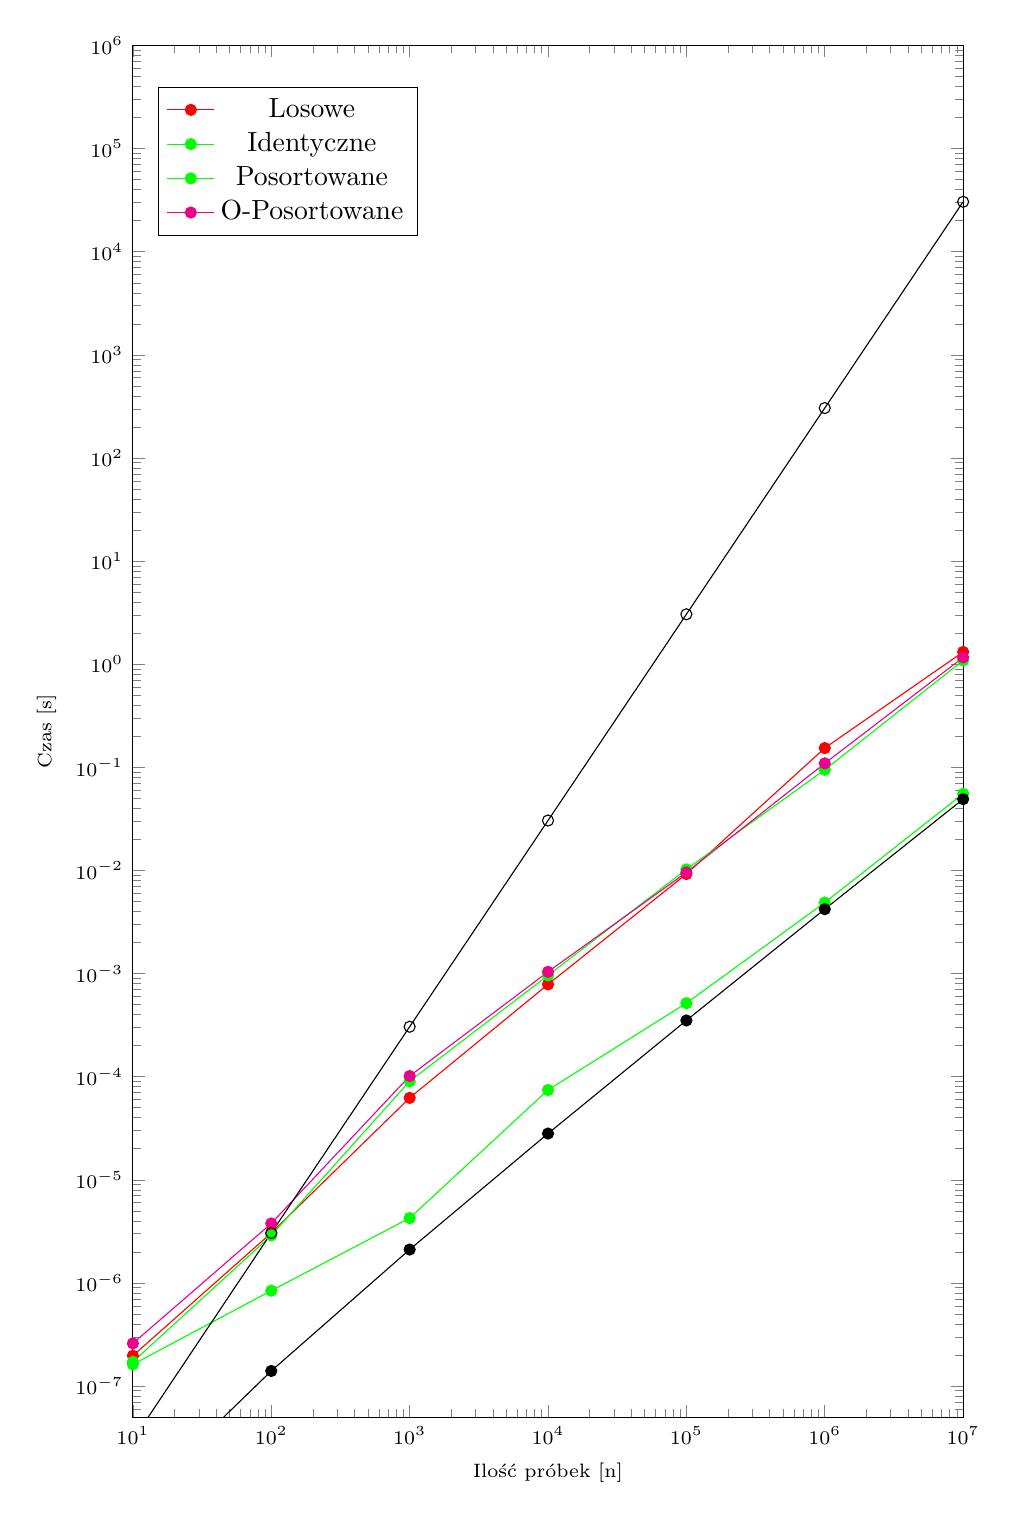
\begin{tikzpicture}
\\
\begin{axis}[
    width=\textwidth,
    height=19cm,
    legend pos=north west,
	xmode = log,
	ymode = log,
	xlabel={Ilość próbek [n]},
	ylabel={Czas [s]},
	xmin=10,xmax=10000000,
	ymin= 0.00000005, ymax=1000000,
	label style={font=\scriptsize},
	tick label style={font=\scriptsize},
	minor y tick num=1
]

\addplot[color=red,mark=*]
coordinates {
(10,0.0000001969 )
(100,0.0000030504)
(1000,0.0000622609)
(10000,0.0007856392)
(100000,0.0092356374)
(1000000,0.1538449949)
(10000000,1.3153185818)
};

\addplot[color=green,mark=*]
coordinates {
(10,0.0000001621 )
(100,0.0000008411)
(1000,0.0000042528)
(10000,0.0000743194)
(100000,0.0005163060)
(1000000,0.0048810180)
(10000000,0.0553684626)
};

\addplot[color=green,mark=*]
coordinates {
(10,0.0000001717 )
(100,0.0000028876)
(1000,0.0000903414)
(10000,0.0009601499)
(100000,0.0102522893)
(1000000,0.0947384417)
(10000000,1.0889244169)
};

\addplot[color=magenta,mark=*]
coordinates {
(10,0.0000002591 )
(100,0.0000037742)
(1000,0.0001014180)
(10000,0.0010400160)
(100000,0.0095718207)
(1000000,0.1092921324)
(10000000,1.1636245519)
};

\addplot[color=black,mark=*]
coordinates {
(10,0.000000007 )
(100,0.000000140)
(1000,0.000002107)
(10000,0.000028091)
(100000,0.000351138)
(1000000,0.004213657)
(10000000,0.049159335)
};

\addplot[color=black,mark=o]
coordinates {
(10,0.000000030 )
(100,0.000003050)
(1000,0.000304995)
(10000,0.030499469)
(100000,3.049946857)
(1000000,304.994685714)
(10000000,30499.468571429)
};

\legend{Losowe, Identyczne,Posortowane, O-Posortowane, }
\end{axis}
\end{tikzpicture}

\section{Algorytm Hybrid Sort }
\subsection{Opis}
Jest to algorytm Quick Sort rozszerzony o sortowanie przy użyciu Insertion Sort podtablic gdy ich długość nie przekrasza 60 elementów. 
\subsection{Tabela pomiarów}

\begin{center}
\begin{tabular}{lcccc}  
\\
\toprule
Rozmiar[n] & \multicolumn{4}{c}{Czas[s]} \\
\cmidrule(r){2-5}
 & Losowe & Posortowane & O-Posortowane & Identyczne \\
\midrule
10       & 0.0000000779  & 0.0000000928 & 0.0000000972  & 0.0000000854 \\
100      & 0.0000005448  & 0.0000002899 & 0.0000005039  & 0.0000004741 \\
1000     & 0.0000104756  & 0.0000079857 & 0.0000081701  & 0.0000065568 \\
10000    & 0.0001202881  & 0.0000716271 & 0.0003220885  & 0.0001679542 \\
100000   & 0.0015019490  & 0.0011353100 & 0.0013169724  & 0.0013053846 \\
1000000  & 0.0389635356  & 0.0124492272 & 0.0163029062  & 0.0164278488 \\
10000000 & 0.2409883819  & 0.1682131104 & 0.1682539896  & 0.1864922700 \\
\bottomrule
\end{tabular}
\end{center}

\subsection{Wykres}

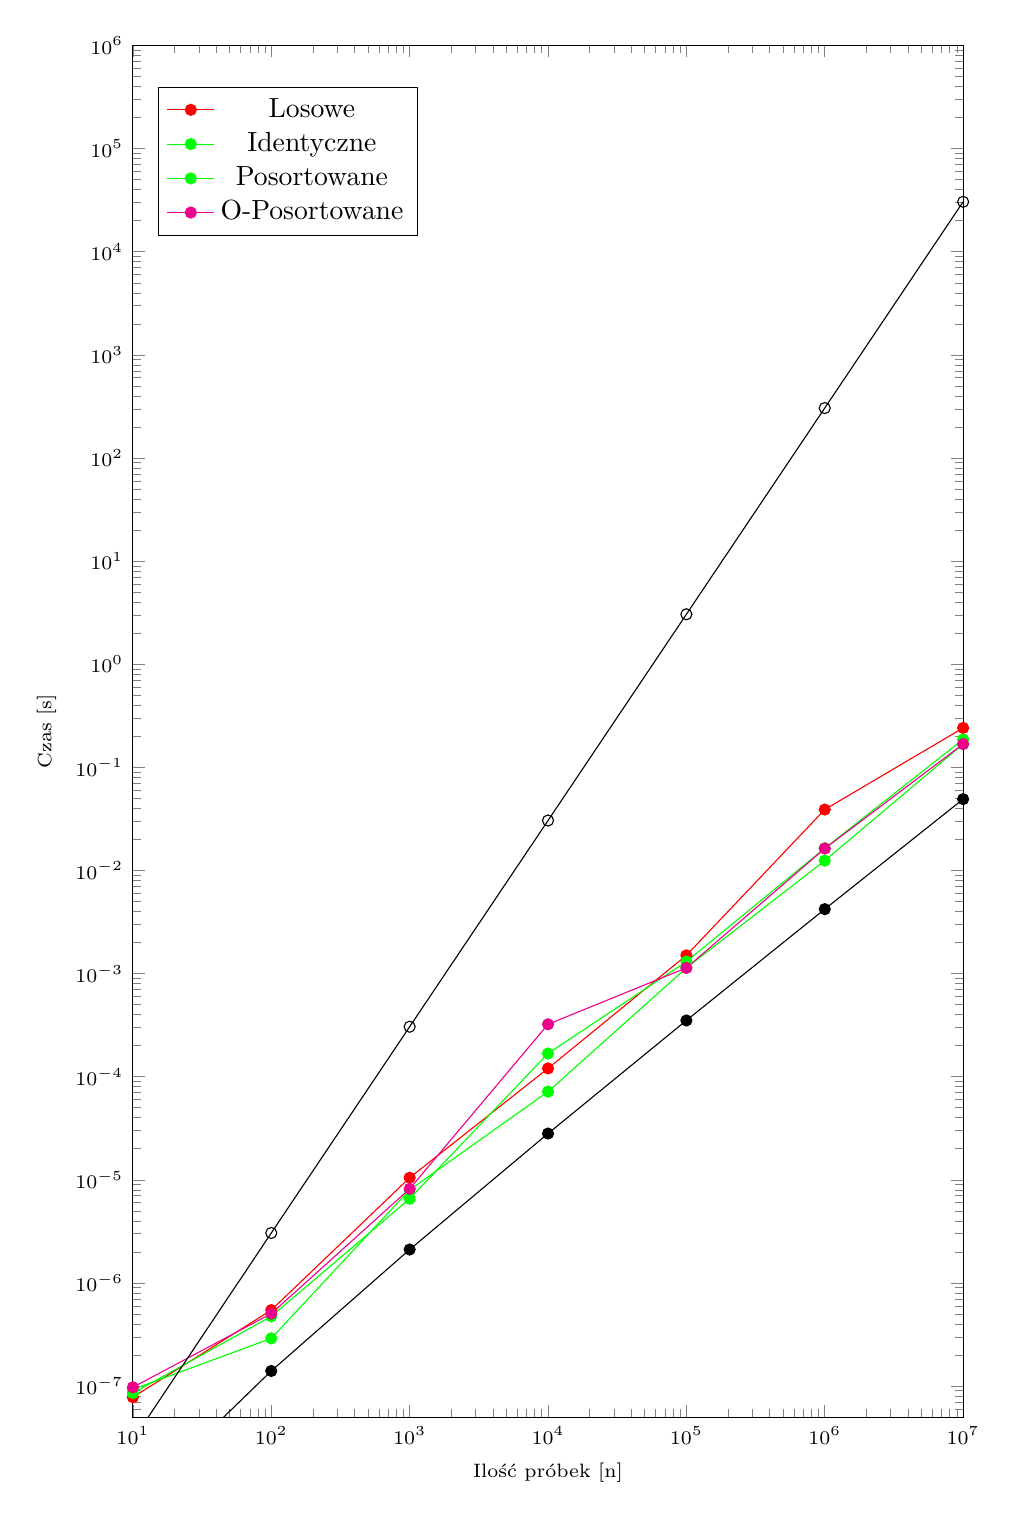
\begin{tikzpicture}
\\
\begin{axis}[
    width=\textwidth,
    height=19cm,
    legend pos=north west,
	xmode = log,
	ymode = log,
	xlabel={Ilość próbek [n]},
	ylabel={Czas [s]},
	xmin=10,xmax=10000000,
	ymin= 0.00000005, ymax=1000000,
	label style={font=\scriptsize},
	tick label style={font=\scriptsize},
	minor y tick num=1
]

\addplot[color=red,mark=*]
coordinates {
(10,0.0000000779 )
(100,0.0000005448)
(1000,0.0000104756)
(10000,0.0001202881)
(100000,0.0015019490)
(1000000,0.0389635356)
(10000000,0.2409883819)
};

\addplot[color=green,mark=*]
coordinates {
(10,0.0000000854 )
(100,0.0000004741)
(1000,0.0000065568)
(10000,0.0001679542)
(100000,0.0013053846)
(1000000,0.0164278488)
(10000000,0.1864922700)
};

\addplot[color=green,mark=*]
coordinates {
(10,0.0000000928 )
(100,0.0000002899)
(1000,0.0000079857)
(10000,0.0000716271)
(100000,0.0011353100)
(1000000,0.0124492272)
(10000000,0.1682131104)
};

\addplot[color=magenta,mark=*]
coordinates {
(10,0.0000000972 )
(100,0.0000005039)
(1000,0.0000081701)
(10000,0.0003220885)
(100000,0.0011353100)
(1000000,0.0163029062)
(10000000,0.1682131104)
};

\addplot[color=black,mark=*]
coordinates {
(10,0.000000007 )
(100,0.000000140)
(1000,0.000002107)
(10000,0.000028091)
(100000,0.000351138)
(1000000,0.004213657)
(10000000,0.049159335)
};

\addplot[color=black,mark=o]
coordinates {
(10,0.000000030 )
(100,0.000003050)
(1000,0.000304995)
(10000,0.030499469)
(100000,3.049946857)
(1000000,304.994685714)
(10000000,30499.468571429)
};

\legend{Losowe, Identyczne,Posortowane, O-Posortowane, }
\end{axis}
\end{tikzpicture}

\section{Wnioski}
Pomiary zostały przeprowadzone na komputerze z procesorem 
i5-6300U o częstotliwości pracy 2.40Ghz.\\
Wielkość danych wejściowych zaczynała się od $10$ do $10^7$
Badane były 4 typy danych wejściowych:
\begin{itemize}  
\item Liczbny losowe  $x \in (1 ... n)$
\item Liczby identyczne  
\item Liczby posortowane 
\item Liczby posortowane  odwrotnie 
\end{itemize}

Pomiary zostały uśrednione z 5 powtórzeń.
Najszybszy okazał się Hybrid Sort.
Quick Sort po przez odpowieni dobór Pivota nie ogiągnął pesymistycznego przypadku.
Najwolniejszym algorytmem okazał się Heap Sort, jedynie dla danych identycznych był zdecydowanie najszybszy.

\end{document}